\documentclass[main.tex]{subfiles}
\usepackage{tikz-feynman}
\begin{document}
\chapter{Assorted}
In this chapter I include a bunch of really important things that aren't long enough to fit into a chapter of their own.

Other stuff I want to add:
\begin{enumerate}
\item Background gauge fields. Maybe put in the section on Feynman diagrams?  I see how hard it is to organize any presentation of 

\item Feynman parameters. Good resource: \url{http://hitoshi.berkeley.edu/229A/self-energy.pdf}, labeled feynmanparameters.pdf in my academicstuff folder. 

In the feynman parameters, introduce it abstractly, then shwo how to do it in a kleingordon case, then do it in a QED calculation.
\end{enumerate}
\section{Diagrams}
Just testing feynman diagrams. $\Pi_2$ photon loop. Using tikz picture:
\begin{equation}
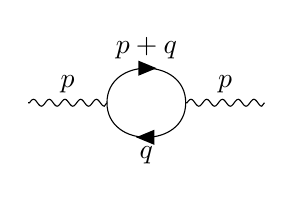
\begin{tikzpicture}
\begin{feynman}
\vertex (a1);
\vertex[right=1cm of a1] (a2);
\vertex[right=1cm of a2] (a3) ;
\vertex[right=1cm of a3] (a4);

\diagram* {
(a1) -- [boson,edge label=\(p\)] (a2),
(a2) -- [fermion, half left, edge label=\(p+q\)] (a3),
(a3) -- [fermion, half left,edge label=\(q\)] (a2),
(a3) -- [boson, edge label=\(p\)] (a4),
};
\end{feynman}
\end{tikzpicture}
=2
\end{equation}
Using equation with tikz-feynman document:
\begin{equation}
\feynmandiagram [baseline=(d.base)] {
a -- [fermion] b -- [fermion] c,
b -- [boson] d [particle=\(\gamma\)],
};
= i g_{e} \gamma^{\mu}
\end{equation}
Using equation with format from tikzpicture:


\end{document}